\documentclass[aspectratio=169,11pt,t]{beamer}
% ============================================================
%  ksa-cs-v2: ksa-cs-lecture-template.tex 스타일 + 한글, v2 덱(16:9)용.
%    - 짙은 네이비 헤드라인 (섹션 이름 + 프레임마다 점)
%    - 꽉 찬 파란 제목 막대, 둥근 그림자 블록
%    - 한글: Noto Sans CJK KR (fontspec)
%  사용:
%    \documentclass[aspectratio=169,11pt,t]{beamer}
%    \input{<..>/theme/ksa-cs-v2.tex}
%  ksa-theme.tex 의 매크로(\kb \kq, ksablue/ksared 등)도 같은 이름으로 둔다
%  -> v2 덱 본문을 거의 그대로 옮길 수 있다.
% ============================================================

\usepackage{fontspec}
\usepackage{amsmath,amssymb}
\usepackage{tikz}
\usepackage{listings}
\usepackage{graphicx}
\usepackage{booktabs}
\usepackage{varwidth}
% enumitem 은 넣지 않는다 (beamer 글머리표가 사라진다)

\defaultfontfeatures{Ligatures=TeX}
\setmainfont{Noto Sans CJK KR}
\setsansfont{Noto Sans CJK KR}
\setmonofont{Noto Sans Mono CJK KR}[Scale=0.92]
\usefonttheme{professionalfonts}

% ---------- 기본 틀 ----------
\usetheme{default}
\useinnertheme[shadow=true]{rounded}
\setbeamertemplate{navigation symbols}{}
\setbeamersize{text margin left=1em,text margin right=1em}

% ---------- 색 (템플릿 원본 값) ----------
\definecolor{navydark}{HTML}{191959}
\definecolor{navydim}{HTML}{8888B0}
\definecolor{navytitle}{HTML}{262686}
\definecolor{navyblue}{HTML}{3333B2}
\definecolor{blockbodybg}{HTML}{E9E9F3}
\definecolor{examplegreen}{HTML}{006000}
\definecolor{examplebg}{HTML}{E5EFE5}
\definecolor{alertred}{HTML}{BF0000}
\definecolor{alertbg}{HTML}{F9E5E5}
% ksa-theme.tex 와 같은 이름 (본문 호환)
\colorlet{ksablue}{navytitle}
\colorlet{ksabluedk}{navydark}
\definecolor{ksagold}{HTML}{D6CBB1}
\definecolor{ksagolddk}{HTML}{A9976B}
\colorlet{ksared}{alertred}
\definecolor{ksagray}{HTML}{5B5B5B}

\setbeamercolor{structure}{fg=navyblue}
\setbeamercolor{alerted text}{fg=alertred}
\setbeamercolor{frametitle}{bg=navytitle,fg=white}
\setbeamercolor{title}{fg=white,bg=navytitle}
\setbeamercolor{block title}{bg=navytitle,fg=white}
\setbeamercolor{block body}{bg=blockbodybg,fg=black}
\setbeamercolor{block title example}{bg=examplegreen,fg=white}
\setbeamercolor{block body example}{bg=examplebg,fg=black}
\setbeamercolor{block title alerted}{bg=alertred,fg=white}
\setbeamercolor{block body alerted}{bg=alertbg,fg=black}
\setbeamercolor{item}{fg=navyblue}
\setbeamertemplate{itemize item}[circle]
\setbeamertemplate{itemize subitem}[triangle]

% ---------- 헤드라인: miniframes (섹션 이름 + 점) ----------
\useoutertheme[subsection=false]{miniframes}
\setbeamerfont{section in head/foot}{size=\tiny}
\setbeamercolor{section in head/foot}{bg=navydark,fg=white}
\setbeamercolor{mini frame}{fg=white}
\setbeamertemplate{mini frames}[circle]

% ---------- 제목 막대: 폭 꽉 채움, 두 줄까지 ----------
\setbeamerfont{frametitle}{size=\normalsize,series=\bfseries}
\setbeamertemplate{frametitle}{%
  \nointerlineskip
  \begin{beamercolorbox}[wd=\paperwidth,ht=2.7ex,dp=1.1ex,leftskip=.3cm,rightskip=.3cm]{frametitle}%
    \usebeamerfont{frametitle}\insertframetitle
  \end{beamercolorbox}}

% ---------- 쪽 번호: 오른쪽 아래 ----------
\setbeamertemplate{footline}{%
  \hfill
  {\color{navydim}\scriptsize\insertframenumber\,/\,\inserttotalframenumber}%
  \hspace{3mm}\vspace{2mm}%
}

% ---------- 표지: 템플릿처럼 헤드라인은 그대로, 가운데 둥근 그림자 상자에 제목 한 줄 ----------
% 덱에서:  {\setbeamertemplate{footline}{}\begin{frame}[c,noframenumbering]\titlepage\end{frame}}
\setbeamercolor{title}{fg=white,bg=navyblue}
\makeatletter
\setbeamertemplate{title page}{%
  \vfill
  \centering
  \begin{minipage}{0.84\paperwidth}
  \begin{beamercolorbox}[wd=\linewidth,sep=7pt,center,rounded=true,shadow=true]{title}
    {\usebeamerfont{title}\inserttitle\par}%
    \ifx\insertsubtitle\@empty\else\vskip0.4em{\usebeamerfont{subtitle}\insertsubtitle\par}\fi
  \end{beamercolorbox}
  \end{minipage}\par\vskip1.6em
  {\usebeamerfont{author}\color{navytitle}\insertauthor\par}\ifx\beamer@date\@empty\vskip0.3em\else\vskip1.3em\fi
  {\usebeamerfont{institute}\color{ksagray}\insertinstitute\par}%
  \ifx\beamer@date\@empty\else\vskip0.3em{\usebeamerfont{date}\color{ksagray}\insertdate\par}\fi
  \vfill
}
\makeatother
\setbeamerfont{title}{series=\bfseries,size=\Large}
\setbeamerfont{subtitle}{size=\normalsize}
\setbeamerfont{author}{size=\normalsize}
\setbeamerfont{institute}{size=\small}
\setbeamerfont{date}{size=\small}

% ksa-theme 호환: 덱이 \renewcommand{\ksacredit}{..} 를 해도 되게 (꼬리말에는 안 쓴다)
\newcommand{\ksacredit}{}

% ---------- 강조 ----------
\newcommand{\hl}[1]{\textcolor{alertred}{#1}}
\newcommand{\hlb}[1]{\textcolor{navyblue}{#1}}
\newcommand{\kb}[1]{\textbf{\color{ksablue}#1}}
\newcommand{\kq}[1]{\textbf{\color{ksared}#1}}

% ---------- 파이썬 코드 (템플릿과 같은 색) ----------
\definecolor{codekw}{HTML}{0033B3}
\definecolor{codebuiltin}{HTML}{BF0000}
\definecolor{codestr}{HTML}{067D17}
\definecolor{codecomment}{HTML}{8C8C8C}
\definecolor{codenum}{HTML}{1750EB}
\lstdefinestyle{py}{
  language=Python, basicstyle=\ttfamily\scriptsize,
  keywordstyle=\color{codekw}\bfseries, stringstyle=\color{codestr},
  commentstyle=\color{codecomment}\itshape, numberstyle=\color{codenum},
  emph={print,len,range,sum,input,int,str,float,list,dict,append,remove,sorted,abs,min,max},
  emphstyle=\color{codebuiltin}, showstringspaces=false, keepspaces=true,
  columns=fixed, basewidth=0.52em, aboveskip=1mm, belowskip=1mm, xleftmargin=2mm,
  breaklines=true
}
\lstset{style=py}

% 원본 덱 (ksa-theme) 의 그림·실습은 이 폴더로 합쳤다 (옛 원본: slides/old/v2/)
\setbeamerfont{author}{size=\normalsize}
\setbeamerfont{institute}{size=\small}
\graphicspath{{figs/}{../../../assets/}}
\makeatletter
\newcommand{\markpage}[1]{\protected@write\@auxout{}{\string\newlabel{#1}{{\the\c@framenumber}{}}}\hypertarget{#1}{}}
\newcommand{\pref}[1]{\hyperlink{#1}{\textcolor{ksagolddk}{(p.\ref{#1})}}}
\makeatother
% 야구 숫자 (exp_baseball.py → assets/baseball.json 에서 옮겨 적었고 data.py 가 같은지 확인한다)
% 투구: 2024-06 MLB 정규시즌 모든 투구 (Baseball Savant), 한 행 = 공 하나
\newcommand{\hrN}{116{,}355}      % 투구 수
\newcommand{\hrPos}{921}          % 홈런이 된 공
\newcommand{\hrNo}{115{,}434}     % 홈런이 아닌 공
\newcommand{\hrRate}{0.79}        % 홈런 비율 (%)
\newcommand{\hrAccZero}{99.21}    % 전부 '홈런 아님' 정확도 (%)
\newcommand{\hrOhP}{498}\newcommand{\hrOhHR}{12}   % 6월 오타니가 받은 공 · 홈런
\newcommand{\hrPA}{30{,}060}\newcommand{\hrPArate}{3.06}\newcommand{\hrPerPA}{3.87}   % 타석 수 · 타석당 홈런 비율 · 타석당 공
\newcommand{\hrBat}{480}\newcommand{\hrBatHR}{310}\newcommand{\hrBatRate}{64.6}   % 타자 수 · 6월에 홈런을 친 타자
% 규칙: 던지기 직전 볼카운트가 3-1 또는 3-2 이면 '홈런'
\newcommand{\paAccRule}{92.39}\newcommand{\paCalled}{8{,}189}
\newcommand{\paTP}{126}\newcommand{\paFP}{8{,}063}\newcommand{\paFN}{795}
\newcommand{\paPrec}{1.54}\newcommand{\paRec}{13.7}
% 던지기 전 두 문제: 같은 투구 (구속 · 구종 있는 공), 6/1~23 학습 · 6/24~30 시험, 입력 = 볼카운트 · 타자 · 투수
\newcommand{\prN}{115{,}940}\newcommand{\prTrain}{88{,}024}\newcommand{\prTest}{27{,}916}\newcommand{\prSwing}{48.2}
\newcommand{\prAccBase}{51.4}\newcommand{\prAccCount}{59.6}\newcommand{\prAccModel}{60.3}
\newcommand{\canTwo}{1.6}\newcommand{\canTop}{2.1}\newcommand{\canMax}{5.2}   % 3-2 홈런 비율 · 홈런 타자 상위 10% · 모델 최대 확률 (%)
\newcommand{\prMean}{143.6}\newcommand{\prMaeBase}{8.0}\newcommand{\prMaeModel}{7.3}\newcommand{\prMaeLeak}{2.3}

\renewcommand{\ksacredit}{Machine Learning and Deep Learning \,\textperiodcentered\, 문제 정형화와 평가지표}
\title{문제 정형화와 평가지표}
\subtitle{Problem Formulation · Metrics · Baselines}
\author{Machine Learning and Deep Learning}
\institute{KSA 2027-Spring}
\date{Sumin Han (suminhan@ksa.hs.kr)}
\begin{document}
{\setbeamertemplate{footline}{}\begin{frame}[c,noframenumbering]\titlepage\end{frame}}

\section{질문}
% --- 오늘의 질문
\begin{frame}{오늘의 질문}
\vfill
\begin{columns}[c]
\begin{column}{0.5\textwidth}
\centering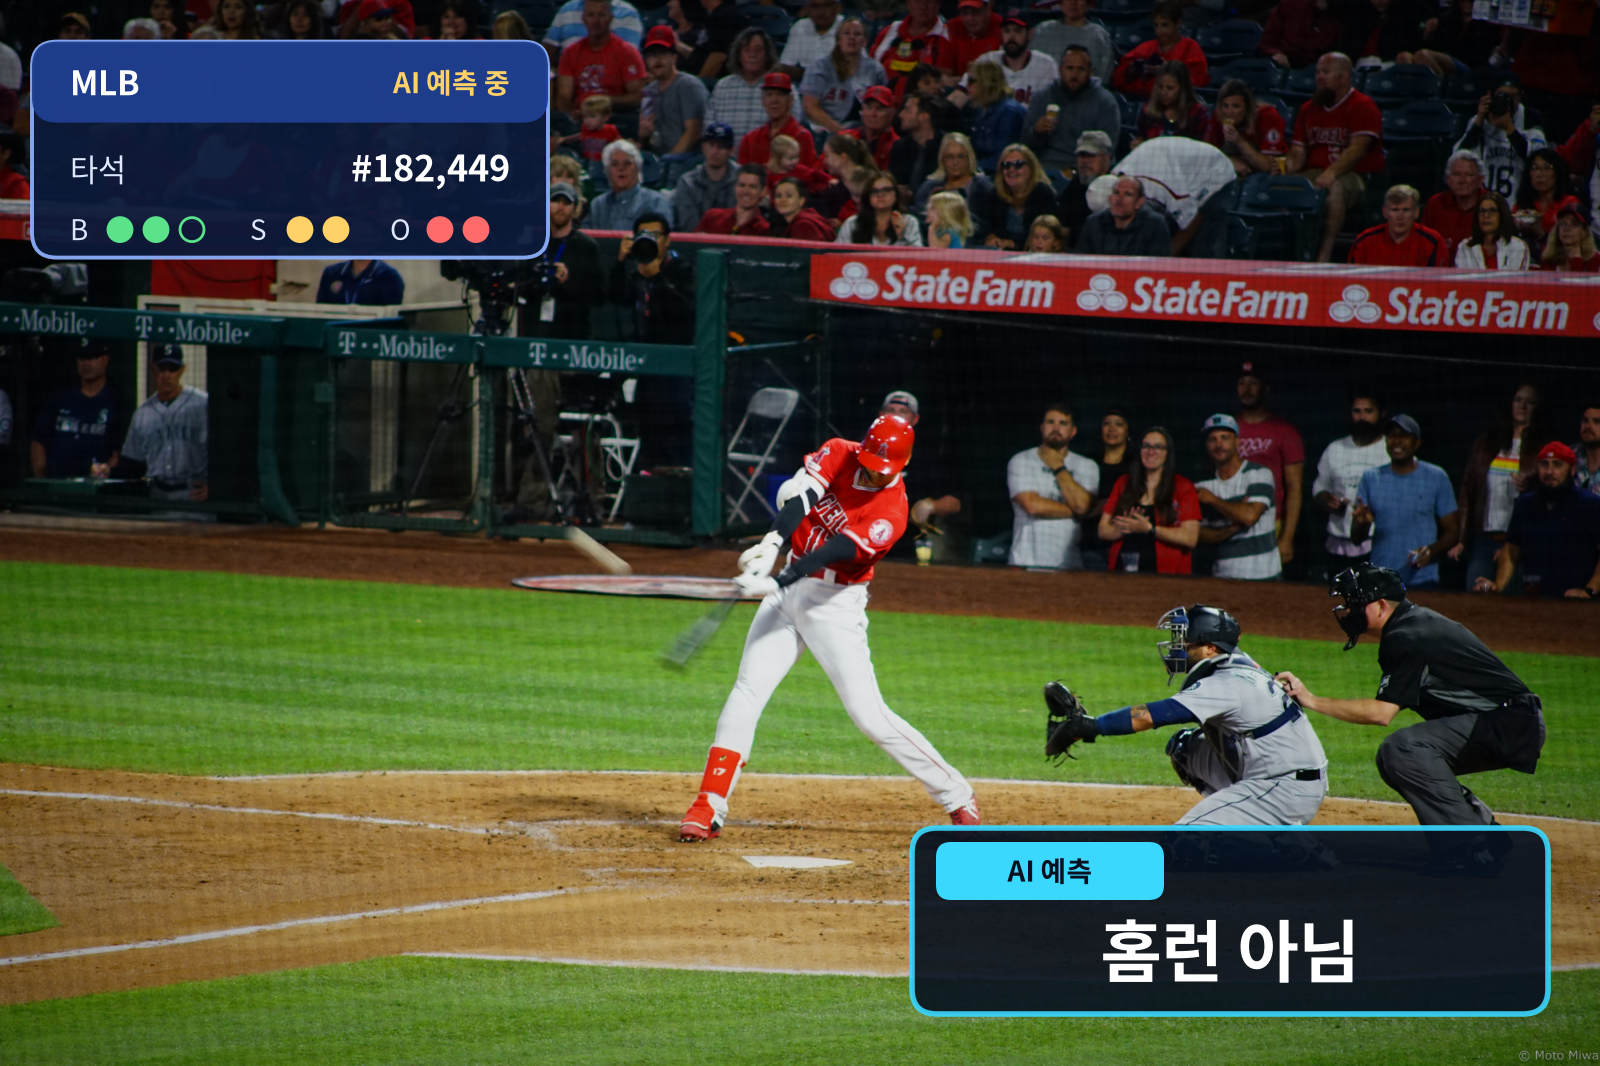
\includegraphics[width=\linewidth]{pf_homerun}
\end{column}
\begin{column}{0.48\textwidth}
\centering
{\large 투수가 \textbf{공을 던지기 전에},\\ 이번 공이 \textbf{홈런일까?}를 맞히는 \textbf{AI}를 만들었다.}\vskip0.6em
{\large 2024년 6월 MLB 투구 \hrN 개에서}\vskip0.8em
{\fontsize{28}{34}\selectfont\mbox{\textbf{정확도 \kb{\hrAccZero\%}}}}\vskip0.8em
{\Large 좋은 모델일까?}\vskip1.2em
{\small\color{gray} 2024 MLB 정규시즌 6월 (Baseball Savant)}
\end{column}
\end{columns}
\vfill
\note{투수가 공을 던지기 직전에, 이번 공이 홈런이 될지 맞히는 AI를 만들었다고 해 봅시다. 2024년 6월 메이저리그에서 던진 모든 공, \hrN 개에 대해 예측했더니 정확도가 \hrAccZero 퍼센트입니다. 좋은 모델일까요? 잠깐 생각해 봅시다. 99퍼센트면 백 번 중 한 번도 안 틀린다는 뜻인데, 홈런을 잘 맞힌다는 뜻일까요?}
\end{frame}

% --- 답
\begin{frame}{답: 이 AI는 모든 공에 ``홈런 아님''이라고만 했다}
\markpage{answer}
\vfill
\begin{columns}[c]
\begin{column}{0.36\textwidth}
\centering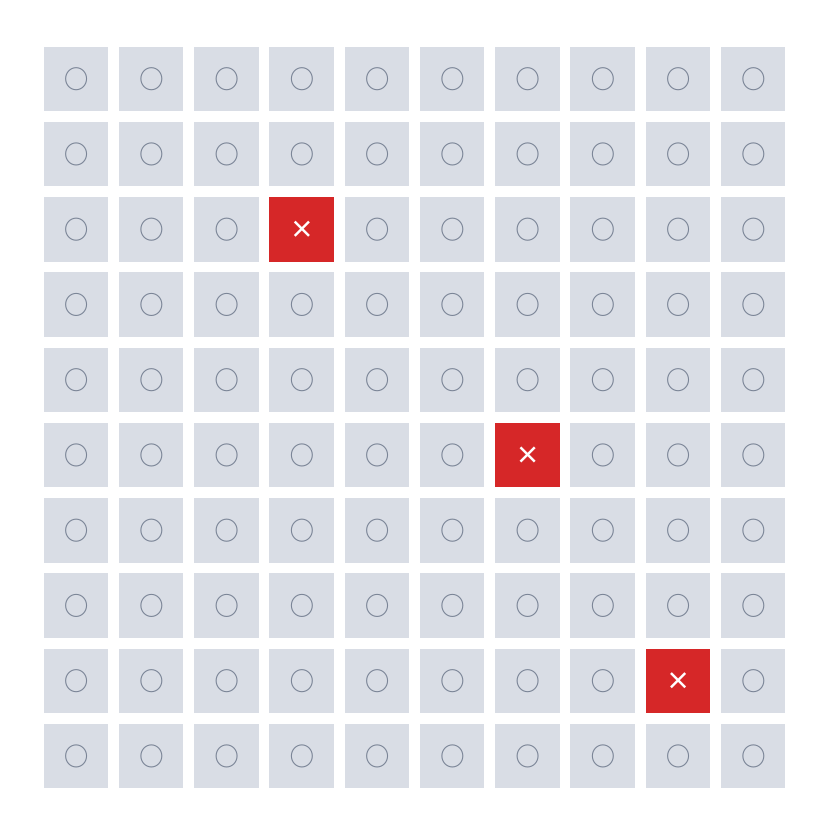
\includegraphics[width=\linewidth]{pf_waffle}\par
{\small 공 100개 중 \textcolor{ksared}{\textbf{홈런 1개}} 꼴 (\hrRate\%)}
\end{column}
\begin{column}{0.6\textwidth}
{\large\renewcommand{\arraystretch}{1.35}
\begin{tabular}{lr}
2024년 6월 MLB 투구 & \hrN\\
\quad 그중 홈런 & \hrPos\ (\hrRate\%)\\
\quad 홈런 아님 & \hrNo\\\hline
맞힌 공 (전부 ``아님'') & \hrNo\\
정확도 & $\dfrac{\hrNo}{\hrN} = \kb{\hrAccZero\%}$\\
잡아낸 홈런 & \kq{0 개}
\end{tabular}}\vskip1em
{\large 홈런이 드물어서 \kq{아무것도 안 해도} 99\%}\\[0.3em]
{\small\color{gray} 6월 오타니가 받은 공 \hrOhP 개 중 홈런 \hrOhHR 개, 하나도 못 맞힌다}
\end{column}
\end{columns}
\vfill
\note{답입니다. 이 AI는 아무것도 하지 않습니다. 모든 공에 홈런 아님이라고만 답합니다. 6월에 던진 공 \hrN 개 중 홈런이 된 공은 \hrPos 개, \hrRate 퍼센트뿐입니다. 그림처럼 공 백 개 중 하나가 될까 말까입니다. 그러니 전부 아님이라고 하면 홈런이 아닌 \hrNo 개를 다 맞히고, 정확도가 \hrAccZero 퍼센트가 됩니다. 대신 홈런은 하나도 못 잡습니다. 오타니는 6월에 공 \hrOhP 개를 받아 홈런 \hrOhHR 개를 쳤는데, 이 AI는 그 \hrOhHR 개를 전부 놓칩니다. 그래서 숫자 하나만 보고 좋은 모델이라고 말할 수 없습니다. 무엇을 맞히는지, 무엇으로 채점하는지, 무엇과 비교하는지를 먼저 정해야 합니다. 오늘은 모델을 만들기 전에 할 일, 문제를 정형화하는 법을 배웁니다. 이 함정은 뒤에서 규칙 하나와 나란히 놓고 다시 봅니다.}
\end{frame}

\section{문제 정하기}
% --- 다섯 칸
\begin{frame}{머신러닝 문제 = 다섯 칸 채우기}
\markpage{five}
\vfill
\centering
{\large
\begin{tabular}{rll}
\kb{①} & \textbf{한 행은 무엇?} & 예시 하나의 단위: 공 하나 (투구), 타석 하나, 타자 한 명\\[0.5em]
\kb{②} & \textbf{입력 $X$} & \textbf{던지기 전} 정보만: 볼카운트 · 타자 · 투수 \kb{O}, 구종 · 비거리 \kq{X}\\[0.5em]
\kb{③} & \textbf{출력 $y$} & 맞히려는 것: 이 공이 홈런? 스윙할까? 구속은?\\[0.5em]
\kb{④} & \textbf{평가지표} & 무엇으로 채점하나: 정확도, MAE, 정밀도 · 재현율 \ldots\\[0.5em]
\kb{⑤} & \textbf{기준선} & 머리 안 쓰는 답의 점수: 가장 흔한 답 (``홈런 아님''), 평균
\end{tabular}}\vskip1.2em
{\large 다섯 칸이 정해져야 \kq{``잘했다''를 말할 수 있다}}
\vfill
\note{머신러닝 문제를 정한다는 건 다섯 칸을 채우는 일입니다. 첫째, 한 행, 즉 예시 하나가 무엇인지. 공 하나인지, 타석 하나인지, 타자 한 명인지. 둘째, 입력. 예측하는 순간에 실제로 알 수 있는 것만 넣어야 합니다. 공을 던지기 직전에 예측한다면, 지금 볼카운트가 몇 볼 몇 스트라이크인지, 누가 치는지, 누가 던지는지는 알 수 있습니다. 하지만 이번 공이 직구인지 변화구인지는 던진 뒤에야 알고, 타구가 몇 미터 날아갔는지는 친 다음에야 압니다. 그걸 입력에 넣으면 답을 미리 보고 맞히는 셈입니다. 셋째, 출력, 맞히려는 것. 넷째, 평가지표, 무엇으로 채점할지. 다섯째, 기준선, 머리를 전혀 안 쓴 답이 몇 점인지. 이 다섯 칸이 정해져야 우리 모델이 잘했다, 못했다를 말할 수 있습니다.}
\end{frame}

% --- 문제 종류
\begin{frame}{출력 $y$ 의 모양이 문제의 종류를 정한다}
\vfill
\centering
{\large
\begin{tabular}{lll}
\textbf{출력 $y$} & \textbf{문제 종류} & \textbf{예}\\[0.2em]\hline\\[-0.6em]
범주 하나 & \kb{분류} (classification) & 이 공이 홈런인가, 스윙할까 (예/아니오)\\[0.5em]
숫자 하나 & \kb{회귀} (regression) & 공의 구속, 타구 비거리
\end{tabular}}\vskip1.2em
{\large 같은 데이터라도 \kq{$y$ 를 무엇으로 정하느냐}에 따라 다른 문제가 된다}
\vfill
\note{출력의 모양이 문제의 종류를 정합니다. 범주 중 하나를 고르면 분류, 숫자 하나를 맞히면 회귀입니다. 이 공이 홈런인가, 타자가 스윙할까는 예 또는 아니오 중 하나를 고르니 분류이고, 공의 구속이나 타구 비거리는 숫자를 맞히니 회귀입니다. 중요한 건, 데이터가 문제를 정하는 게 아니라 우리가 y를 무엇으로 정하느냐가 문제를 정한다는 겁니다. 실제로 해 봅시다.}
\end{frame}

% --- 던지기 전 두 문제
\begin{frame}{같은 공, 두 문제: 스윙할까? 구속은?}
\markpage{batted}
\vfill
\centering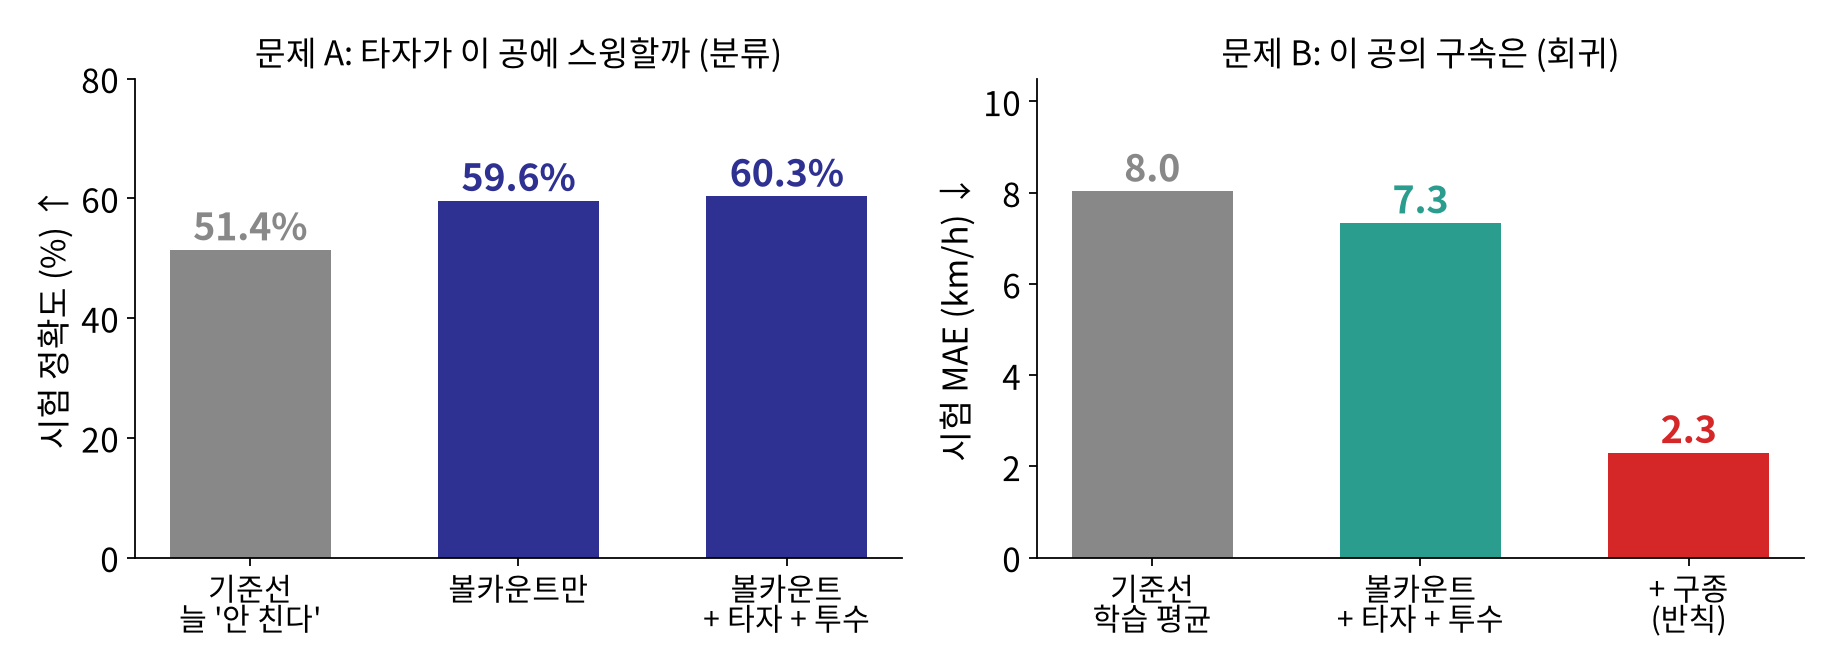
\includegraphics[width=0.8\linewidth]{pf_twoprob.png}\par\vskip0.3em
{\large 문제 A: $y$ = 스윙할까 $\to$ \kb{정확도} \qquad 문제 B: $y$ = 구속 (km/h) $\to$ \kb{MAE}}\\[0.3em]
{\small \kq{구종}은 던진 뒤에야 안다. 넣으면 MAE \prMaeLeak 로 확 줄지만 \kq{반칙}}\\[0.2em]
{\scriptsize\color{gray} 2024년 6월 MLB 투구 \prN 개, 입력 = 던지기 직전 볼카운트 · 타자 · 투수, 6/1$\sim$23 학습 · 6/24$\sim$30 시험, 로지스틱회귀 / 선형회귀}
\vfill
\note{이번에는 같은 투구 데이터로 문제를 두 개 만듭니다. 한 행은 공 하나, 입력은 던지기 직전에 알 수 있는 볼카운트, 타자, 투수입니다. 문제 A는 타자가 이 공에 방망이를 휘두를까를 맞히는 분류, 채점은 정확도입니다. 늘 안 친다고 하면 \prAccBase 퍼센트, 볼카운트만 봐도 \prAccCount 퍼센트, 타자와 투수까지 넣으면 \prAccModel 퍼센트입니다. 3볼 0스트라이크면 거의 안 치고, 3볼 2스트라이크면 대부분 칩니다. 문제 B는 같은 입력으로 이 공의 구속을 맞히는 회귀, 채점은 MAE, 평균 몇 킬로미터 틀렸나입니다. 늘 평균 \prMean 킬로라고 하면 \prMaeBase, 모델은 \prMaeModel 입니다. 생각보다 어렵습니다. 같은 투수라도 직구를 던질지 변화구를 던질지 모르기 때문입니다. 그래서 구종을 입력에 넣으면 \prMaeLeak 로 확 좋아지는데, 이건 반칙입니다. 구종은 공을 던진 뒤에야 알고, 구속을 거의 정해 버리는 답과 같은 정보입니다. 같은 데이터, 다른 y, 다른 지표, 그리고 입력은 예측하는 순간 알 수 있는 것만.}
\end{frame}


% --- 기준선
\begin{frame}{기준선: 머리를 안 쓴 답은 몇 점인가}
\markpage{baseline}
\vfill
\centering
{\large
\begin{tabular}{lll}
\textbf{문제} & \textbf{기준선} & \textbf{점수}\\[0.2em]\hline\\[-0.6em]
스윙할까 (분류) & 늘 ``안 친다''라고 답 & 정확도 \kq{\prAccBase\%}\\[0.5em]
구속 (회귀) & 늘 학습 데이터의 평균 구속 (\prMean km/h) & MAE \kq{\prMaeBase km/h}\\[0.5em]
모든 공 (분류) & 늘 ``홈런 아님''이라고 답 & 정확도 \kq{\hrAccZero\%}
\end{tabular}}\vskip1.2em
{\large 모델 점수는 \kb{기준선과 비교}해서 읽는다}
\vfill
\note{기준선은 머리를 전혀 쓰지 않은 답입니다. 분류면 늘 가장 흔한 답, 회귀면 늘 학습 데이터의 평균. 스윙 문제는 기준선이 \prAccBase 퍼센트라서, 모델의 \prAccModel 퍼센트는 동전 던지기보다 꽤 낫습니다. 구속은 늘 평균이라고 해도 \prMaeBase 킬로밖에 안 틀려서, 모델의 \prMaeModel 은 조금 나을 뿐입니다. 모든 공에 홈런이냐를 물으면 기준선이 \hrAccZero 퍼센트, 처음 본 그 AI의 점수입니다. 같은 높은 정확도라도 기준선에 따라 의미가 정반대입니다.}
\end{frame}

% --- 시험은 미래
\begin{frame}{시험 데이터 = 모델이 ``실제로 만날'' 데이터}
\vfill
\centering
{\large
\begin{tabular}{ll}
\textbf{나누는 법} & \textbf{결과}\\[0.2em]\hline\\[-0.6em]
무작위로 섞기 & \kq{X}: 같은 경기 · 같은 타석의 앞뒤 공이 학습과 시험에 나뉜다\\[0.5em]
\kb{날짜 순서대로} & \kb{O}: 6월 1$\sim$23일로 학습, 24$\sim$30일로 시험 (오늘 쓰는 두 문제 모두)
\end{tabular}}\vskip1.2em
{\large 미래를 섞어 학습하면 \kq{시험 점수가 거짓말}을 한다}
\vfill
\note{평가지표만큼 중요한 게 어떤 데이터로 채점하느냐입니다. 시험 데이터는 모델이 실제로 쓰일 때 만날 데이터를 흉내 내야 합니다. 앞으로 열릴 경기의 공을 예측하는 모델이라면 늘 과거로 미래를 맞힙니다. 그래서 6월 23일까지로 학습하고 그 뒤 일주일로 시험해야 합니다. 무작위로 섞으면 같은 경기, 같은 타석의 바로 앞뒤 공이 학습과 시험에 나뉘어 들어가서, 미래를 엿본 셈이 되고 시험 점수가 실제보다 좋게 나옵니다.}
\end{frame}

\section{한 행과 지표}





% --- 한 행을 무엇으로
\begin{frame}{한 행을 무엇으로 정하나: 공 vs 타석 vs 타자}
\vfill
\centering
{\large\renewcommand{\arraystretch}{1.25}
\begin{tabular}{llll}
& \textbf{한 행 = 공 하나} & \textbf{타석 하나} & \textbf{타자 한 명}\\\hline
행 수 & \hrN & \hrPA & \hrBat\\
$y = 1$ 인 행 & \hrPos & \hrPos & \hrBatHR\\
홈런 비율 & \kq{\hrRate\%} & \hrPArate\% & \kb{\hrBatRate\%}\\
현실의 질문 & 이 공이 홈런? & 이 타석이 홈런? & 이 타자가 이번 달 홈런?
\end{tabular}}\vskip1.2em
{\large 같은 기록, 다른 문제. ``홈런 비율''이 숫자마다 다른 이유}\\[0.3em]
{\small\color{gray} 2024년 6월 MLB. 타석은 홈런으로 끝났으면 1, 타자는 6월에 홈런을 한 번이라도 쳤으면 1}
\vfill
\note{다섯 칸의 첫 칸, 한 행을 무엇으로 정하느냐도 문제를 바꿉니다. 같은 6월 기록입니다. 공 하나를 한 행으로 보면 홈런 비율은 \hrRate 퍼센트입니다. 타석 하나를 한 행으로, 홈런으로 끝난 타석을 1로 하면 \hrPA 타석 중 \hrPos 개, \hrPArate 퍼센트입니다. 타자 한 명을 한 행으로, 6월에 홈런을 한 번이라도 쳤으면 1로 정하면 \hrBat 명 중 \hrBatHR 명, \hrBatRate 퍼센트가 됩니다. 같은 기록인데 다른 문제입니다. 볼카운트를 입력으로 쓸 수 있는 것도 한 행이 공 하나일 때뿐입니다. 기사나 논문에서 비율을 볼 때, 한 행이 무엇인지부터 확인해야 하는 이유입니다.}
\end{frame}

% --- 지표만 쫓는다
\begin{frame}{지표를 정하면, 모델은 그 지표만 쫓는다}
\vfill
\centering
{\large
\begin{tabular}{ll}
\textbf{지표} & \textbf{이 점수를 최대로 만드는 가장 쉬운 방법}\\[0.2em]\hline\\[-0.6em]
정확도 & 전부 ``홈런 아님'' $\to$ \hrAccZero\%\\[0.5em]
잡은 홈런 수 (재현율) & 전부 ``홈런'' $\to$ 하나도 안 놓침 (그런데 아무 정보가 없다)
\end{tabular}}\vskip1.4em
{\large 지표는 \kq{현실에서 무엇이 손해인지}에서 거꾸로 정한다}\\[0.4em]
{\small\color{gray} 예: 홈런 예측으로 하이라이트 카메라를 미리 돌린다면, 놓친 홈런 장면 하나 vs 헛돌린 카메라 한 번}
\vfill
\note{지표를 하나 정하면 모델은 그 점수만 올리려고 합니다. 정확도만 보면 전부 홈런 아님이라고 하면 됩니다. 반대로 홈런을 몇 개나 잡았나, 이걸 재현율이라고 하는데, 이것만 보면 모든 공에 홈런이라고 하면 하나도 안 놓칩니다. 대신 아무 정보도 없는 예측이죠. 둘 사이의 줄다리기는 3주차에 자세히 봅니다. 그래서 지표는 현실에서 무엇이 손해인지에서 거꾸로 정해야 합니다. 예를 들어 중계 방송이 홈런 예측으로 하이라이트 카메라를 미리 돌린다면, 홈런 장면 하나를 놓치는 손해와 카메라를 헛돌리는 손해 중 무엇이 더 큰가. 이건 수학이 아니라 그 분야의 판단입니다.}
\end{frame}

\section{연습}
% --- 문제풀이
\begin{frame}{문제풀이}
\vfill
\begin{enumerate}
\setlength\itemsep{0.8em}
\item 다섯 칸을 채워 보자: \quad (a) 스팸 문자 거르기 \quad (b) 내일 서울 최고 기온
\item 어떤 타자가 공 1,000개를 받아 홈런 8개를 쳤다. 매번 ``홈런 아님''이라고 하면 정확도는? 잡은 홈런은?
\item 이 공에 스윙할지 맞히는 모델의 입력에 ``구종''을 넣었더니 정확도가 크게 올랐다. 무엇이 잘못됐나?
\item 학생 성적 데이터에서 시험 데이터를 무작위로 뽑았는데, 같은 학생의 다른 학기 기록이 학습 데이터에 있다. 무엇이 문제일까?
\end{enumerate}
\vfill
\note{1번 예시 답. 스팸은 한 행이 문자 하나, 입력은 문자 내용, 출력은 스팸이냐 아니냐, 지표는 스팸이 드물면 정확도 말고 놓친 스팸 수와 잘못 거른 정상 문자 수, 기준선은 전부 정상. 기온은 한 행이 하루, 입력은 오늘까지의 날씨, 출력은 내일 최고 기온, 지표는 평균 몇 도 틀렸나, 기준선은 오늘 기온 그대로. 2번. 정확도 99.2퍼센트, 잡은 홈런 0개. 3번. 구종은 공을 던진 뒤에야 알 수 있는 값입니다. 던지기 전에 예측하는 모델이라면 쓸 수 없습니다. 입력에는 예측하는 순간 알 수 있는 것만 넣어야 합니다. 4번. 같은 학생이 학습과 시험 양쪽에 있으면 모델이 학생을 외워서 맞힙니다. 새 학생에게 쓸 모델이라면 학생 단위로 나눠야 합니다.}
\end{frame}


\section{정리}
% --- 정리
\begin{frame}{정리}
\vfill
\centering\large\begin{tabular}{l}
문제 = \kb{다섯 칸}: 한 행 · 입력 $X$ · 출력 $y$ · 평가지표 · 기준선\\[0.45em]
같은 데이터라도 $y$ 와 \kb{한 행}을 다르게 정하면 다른 문제 (공 vs 타석 vs 타자)\\[0.45em]
점수는 \kq{기준선과 비교}해서 읽는다 (99.21\% 도 ``아무것도 안 함''일 수 있다)\\[0.45em]
시험 데이터는 실제로 만날 데이터처럼: 시간 순서, 사람 · 지역 단위\\[0.45em]
지표는 \kb{현실의 손해}에서 거꾸로 정한다 (놓친 홈런 vs 헛돌린 카메라)
\end{tabular}\par\vskip1.0em
{\large 프로젝트 1 \kq{Abstract}(3주차)에 쓸 것이 바로 이 \kb{다섯 칸}}
\vfill
\note{정리합니다. 머신러닝 문제는 다섯 칸, 한 행, 입력, 출력, 평가지표, 기준선입니다. 같은 데이터라도 y와 한 행을 다르게 정하면 다른 문제가 됩니다. 점수는 반드시 기준선과 비교해서 읽습니다. 시험 데이터는 모델이 실제로 만날 데이터처럼 나눕니다. 지표는 현실에서 무엇이 손해인지에서 거꾸로 정합니다. 그리고 3주차에 내는 프로젝트 1 Abstract에 쓸 것이 바로 이 다섯 칸입니다. 다음 시간에는 데이터를 직접 열어 청소하고 정규화합니다.}
\end{frame}

% --- 출처
\begin{frame}{이미지 · 데이터 출처}
\vfill
\small
\begin{itemize}
\item 투구 (p.1, p.\ref{batted}): Baseball Savant (MLB Statcast), 2024-06 정규시즌 모든 투구 CSV; 게임 화면: 컴투스프로야구2021 (컴투스) 캡처, 아래 자막만 덧그림
\end{itemize}
\vfill
\note{이 덱에 쓴 데이터의 출처입니다.}
\end{frame}
\end{document}
